\documentclass[12pt, oneside]{article}
\usepackage[letterpaper, margin=1in]{geometry}
\usepackage[english]{babel}
\usepackage[utf8]{inputenc}
\usepackage{amsmath}
\usepackage{amsfonts}
\usepackage{amssymb}
\usepackage{tikz}

\usepackage{fancyhdr}
\pagestyle{fancy}
\fancyhf{}
\rhead{Name: \hspace{1.5in} }
\lhead{BECA / Dr. Huson / IB Math SL \\* 4 April 2019 \\* Homework: Regents exponents problems}

\vspace{1cm}

\renewcommand{\headrulewidth}{0pt}

\title{Worksheet and test template}
\author{Chris Huson}
\date{March 2018}

\begin{document}

\subsubsection*{\\* Answer on lined paper. Show work.}

\begin{enumerate}

\vspace{0.5 cm}

\subsubsection*{Rational exponents and radicals}

\item Simplify the expression $\sqrt[3]{x} \cdot \sqrt[3]{x^5}$

\item If $p(x)=ab^x$ and $r(x)=cd^x$, then $p(x) \cdot r(x)$ equals \\*[6pt]
(1) $ac(b+d)^x$ \, \qquad (3) $ac(bd)^x$\\*
(2) $ac(b+d)^{2x}$ \qquad (4) $ac(bd)^{x^2}$


\item Simplify the expression $\displaystyle \left( \frac{s^{\frac{2}{3}}}{s^2} \right)^{-\frac{1}{2}}$ to one with positive integer exponents and radicals.

\subsubsection*{Logarithms}
\item What is the inverse of the function $y=\ln x$?


\subsubsection*{Imaginary numbers}
\item Use the quadratic formula to find the solution to the equation $2x^2-4x+7=0$.
\item Simplify the expression $(4+3i)^2$.


\subsubsection*{Polynomial algebra procedures}

\item If $(x-3)$ is a factor of $f(x)=(x-3)(ax^2+bx+c)$, then what is the value of $f(3)$?

\item When $g(x)$ is divided by $x+4$, the remainder is 0. Given $g(x)=x^4+3x^3- 6x^2- 6x-8$. Write down the value of $g(-4)$?\\*[6pt]
("Write down" means by inspection. How can you answer this without calculation?)

\item The velocity of a tidal wave, $v$, in hundreds of miles per hour, can be modeled by the equation $v= 5-\sqrt{t}$, where $t$ represents the time from its origin in hours. Algebraically determine the time when $v=0$.\\*[12pt]
How much faster was the tidal wave traveling after 1 hour than 3 hours, to the \textit{nearest mile per hour}? Justify your answer.


\subsubsection*{Function transformations}
\item Relative to the graph of $y=3 \sin x$, what is the shift of the graph of $y=3 \sin {\left(x- \frac{\pi}{3}\right)}$?

\subsubsection*{Graphing calculator solutions}
\item When $\displaystyle g(x)=\frac{2}{x+2}$ and $h(x)= \log (x+1)+3$ are graphed on the same set of axes, which coordinates best approximate their point of intersection?\\*[6pt]

\item What is the solution to the system of equations $y=3x-2$ and $y=g(x)$ where $g(x)$ is defined by the function below?

\begin{figure}[!ht]
    \centering
    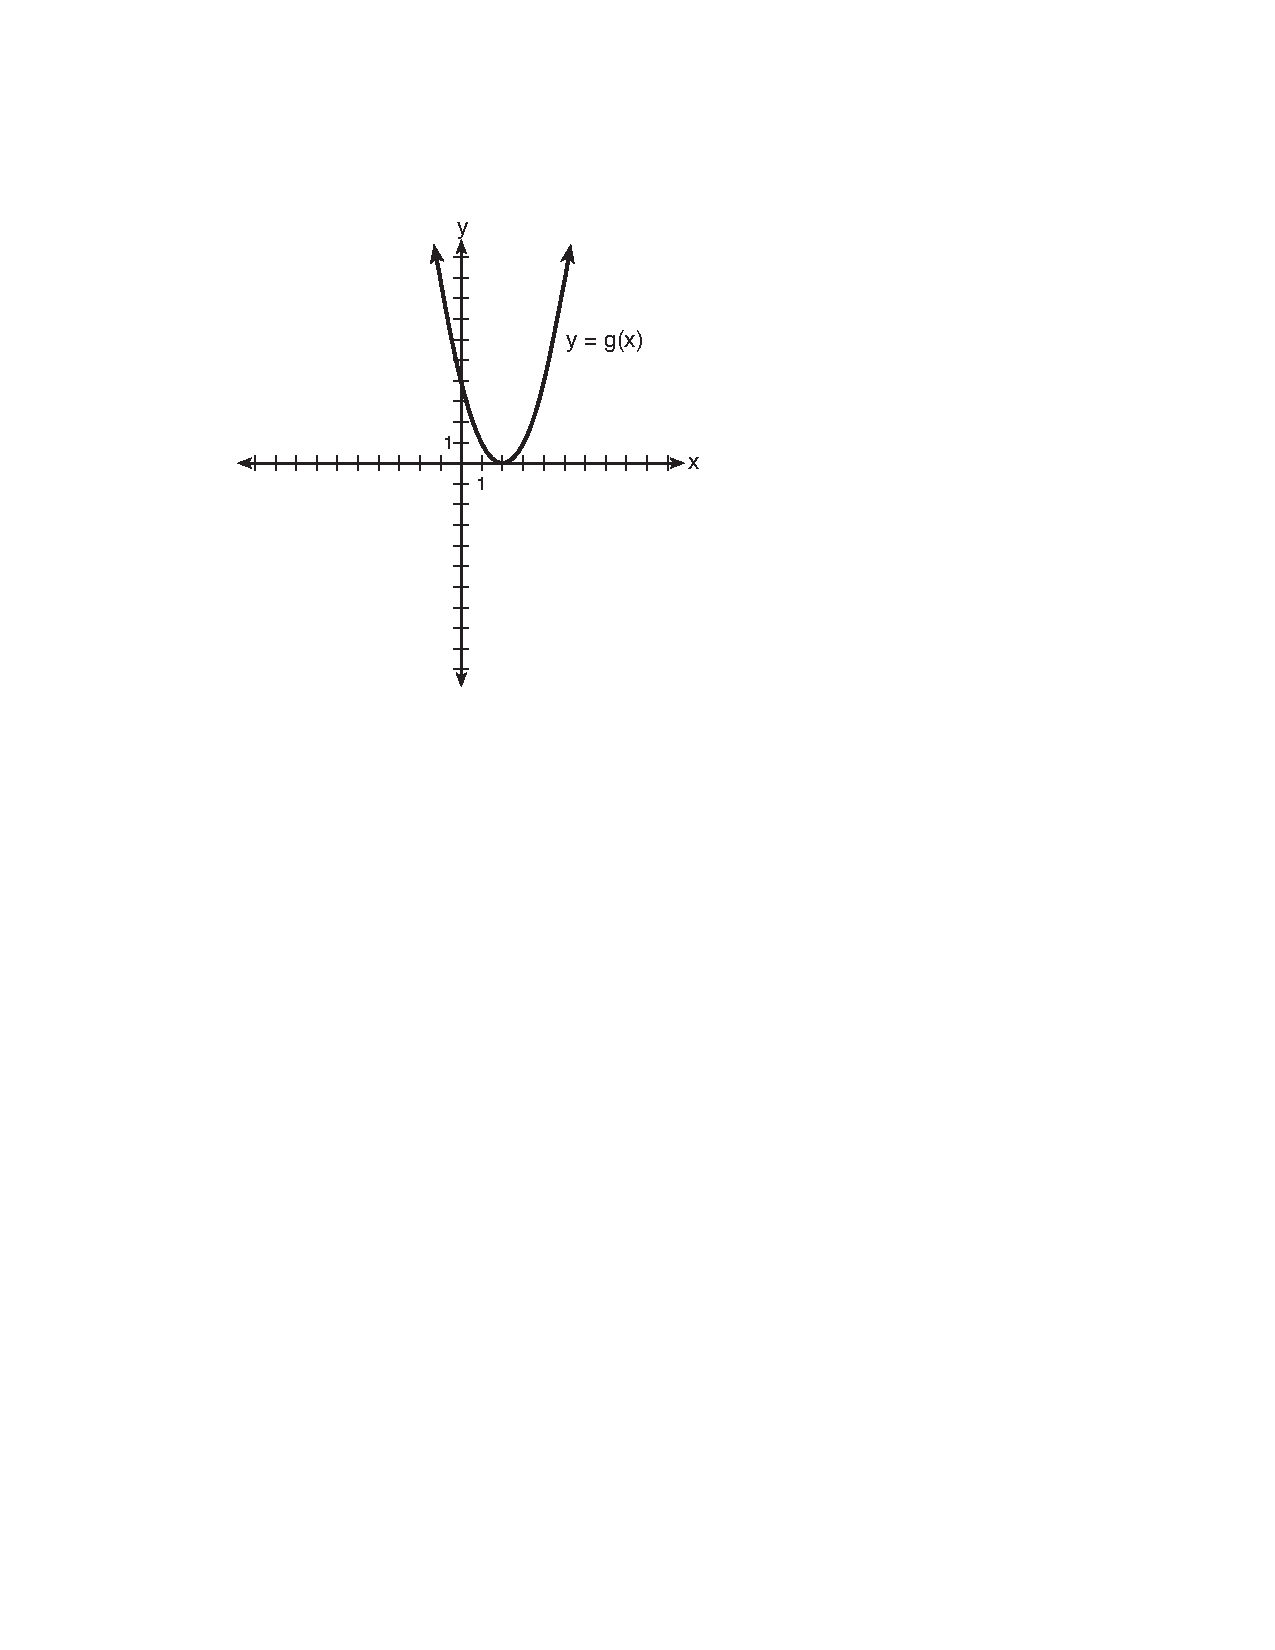
\includegraphics[width=0.4\textwidth]{parabola-graphic.pdf}
\end{figure}


\subsubsection*{Exponential models, base change}
\item A rabbit population doubles every 4 weeks. There are currently five rabbits in a restricted area. If $t$ represents the time, in weeks, and $P(t)$ is the population of rabbits with respect to time, about how many rabbits will there be in 98 days?

\item Pedro and Bobby each own an ant farm. Pedro starts with 100 ants and says his farm is growing exponentially at a rate of 15\% per month. Bobby starts with 350 ants and says his farm is steadily \textit{decreasing} by 5 ants per month.\\*[6pt]
Assuming both boys are accurate in describing the population of their ant farms, after how many months will they both have approximately the same number of ants?\\*[6pt]

\item According to a pricing website, Android phones lose 58\% of their cash value over 1.5 years. Which expression can be used to estimate the value of a \$300 Android phone in 1.5 years?\\*[6pt]
(1) $300e^{-0.87}$ \qquad (3) $300e^{-0.58}$ \\*
(2) $300e^{-0.63}$ \qquad (4) $300e^{-0.42}$


\end{enumerate}
\end{document}
